\subsection{MQ-2: SMOKE SENSOR}
In current technology scenario, monitoring of gases produced is very important. From home appliances such as air conditioners to electric chimneys and safety systems at industries monitoring of gases is very crucial. Gas sensors are very important part of such systems.  Small like a nose, gas sensors spontaneously react to the gas present, thus keeping the system updated about any alterations that occur in the concentration of molecules at gaseous state.\\
Gas sensors are available in wide specifications depending on the sensitivity levels, type of gas to be sensed, physical dimensions and numerous other factors. This Insight covers a methane gas sensor that can sense gases such as ammonia which might get produced from methane. When a gas interacts with this sensor, it is first ionized into its constituents and is then adsorbed by the sensing element. This adsorption creates a potential difference on the element which is conveyed to the processor unit through output pins in form of current. \\
The gas sensor module consists of a steel exoskeleton under which a sensing element is housed. This sensing element is subjected to current through connecting leads. This current is known as heating current through it, the gases coming close to the sensing element get ionized and are absorbed by the sensing element. This changes the resistance of the sensing element which alters the value of the current going out of it.\\
A standard gas sensor module consists of a steel mesh, copper clamping ring and connecting leads. The top part is a stainless steel mesh which takes care of the following:
\begin{enumerate}
\item Filtering out the suspended particles so that only gaseous elements are able to pass to insides of the sensor.  
\item Protecting the insides of the sensor.
\item Exhibits an anti explosion network that keeps the sensor module intact at high temperatures and gas pressures.
\end{enumerate}
\justify The connecting leads of the sensor are thick so that sensor can be connected firmly to the circuit and sufficient amount of heat gets conducted to the inside part. They are casted from copper and have tin plating over them. Four of the six leads (A, B, C, D) are for signal fetching while two (1,2) are used to provide sufficient heat to the sensing element.
\subsubsection{Structure of MQ-2 Gas Sensor}
\begin{figure}[h]
\center
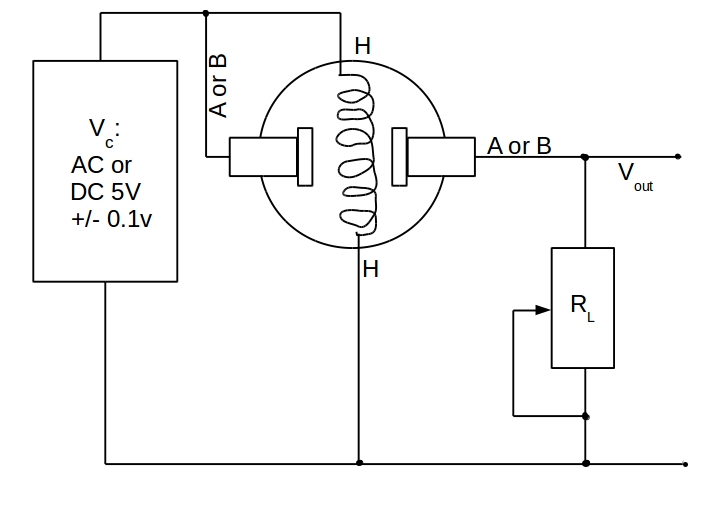
\includegraphics[scale=0.5]{smoke_new.jpg} 
\caption{Structure $\&$ configuration}
\end{figure}
\justify MQ-2 gas sensor has high sensitivity to LPG, Propane and Hydrogen, also could be used to Methane and other combustible steam, it is low cost and suitable for various applications.\\
Using high-quality dual-panel\cite{mq2datasheet} design, with a power indicator and TTL signal output instructions; With a the DO switch signal (TTL) output, and AO analog signal output; TTL output valid signal is low level; (When the low level output signal lights, it can be connected directly to the microcontroller or relay module).\\
TTL output signal can be connected directly to a microcontroller IO port or connect to the relay module, potentiometer is used to adjust the output level transition threshold.
\subsection*{Applications}
They are used in gas leakage detecting equipment in family and industry, are suitable for detecting
of LPG, i-butane, propane, methane ,alcohol, Hydrogen, smoke.
\subsection*{Features}
\begin{enumerate}
\item Wide detecting scope 
\item Fast response and High sensitivity
\item Stable and long life 
\item Simple drive circuit
\item Analog and Digital Outputs
\item Trigger Level configuration Potentiometer 
\end{enumerate}
\subsection*{Technical Specificaations}
\begin{enumerate}
\item Model: FC-22-A
\item Operating voltage: DC 5V
\item Analog Output (AO): 0~5V analog output voltage
\item Digital Outout (DO): 0V or 5V output
\item Configuration: Through Potentiometer (adjusts the output level transition)
\item Preheat Duration: 20s
\end{enumerate}
